\documentclass{article}[11pt]
\usepackage[frenchb,english]{babel}
\usepackage[T1]{fontenc}
\usepackage[utf8]{inputenc}
\usepackage{amsmath,amssymb,latexsym}
\usepackage{times}
\usepackage{float}
\usepackage[left=2cm,right=2cm,top=2cm,bottom=2cm]{geometry}
\frenchbsetup{StandardLists=true} % � inclure si on utilise \usepackage[french]{babel}
\usepackage{enumitem}
\usepackage{fancyhdr}
\usepackage{mathrsfs}
\usepackage{graphicx}
%\usepackage[Algorithme]{algorithm}
%\usepackage{algorithmic}
\usepackage{tikz}
\usepackage{tabularx}
\usetikzlibrary{shapes}
\pagestyle{fancy}
\newcommand{\tr}[1]{{\vphantom{#1}}^{\mathit t}{#1}} 
\renewcommand\headrulewidth{1pt}
\fancyhead[L]{Cours 1�re S}
\fancyhead[R]{Yoann Pietri}
\newcounter{theoremecounter}[subsection]
\usepackage{titlesec}
\setcounter{secnumdepth}{3}% enl�ve la num�rotation apr�s les sections
%\renewcommand\thechapter {\Roman{chapter}}

 \setlength{\parindent}{0pt}

\newcommand{\R}{\mathbb{R}}
\newcommand{\N}{\mathbb{N}}
\newcommand{\Q}{\mathbb{Q}}
\newcommand{\Z}{\mathbb{Z}}
\newcommand{\C}{\mathbb{C}}
\newcommand{\K}{\mathbb{K}}
\newcommand{\eqi}{\Leftrightarrow}
\titleformat{\subsubsection}
   {\normalfont\fontsize{11pt}{13pt}\selectfont\bfseries}% apparence commune au titre et au num�ro
   {\thesubsubsection}% apparence du num�ro
   {1em}% espacement num�ro/texte
   {}% apparence du titre

\tikzstyle{theobox} = [draw=black, very thick,
    rectangle, rounded corners, inner sep=10pt, inner ysep=20pt]
\tikzstyle{theotitle} =[fill=white, text=black,rounded corners,draw=black,very thick]


\usepackage{empheq}
\usepackage[c]{esvect}
\newcommand{\covec}[2]{\begin{pmatrix}#1 \\#2 \end{pmatrix}}

\fancyhead[L]{Sujet : Les matrices}


\begin{document}
\center{Sujets : les matrices}
\flushleft
Si au cours du sujet, le candidat repère ce qui lui semble être une erreur énoncé, il l'indique sur sa copie et continue sa composition. \newline

Il est demandé au candidat une clarté dans les raisonnements qu'il mettra en place. \newline

L'usage de la calculatrice est interdit.\newline

Soit $A$ un ensemble. On définit une loi sur cette ensemble comme une fonction qui à 2 éléments de $A$ associe un élément de $A$ (exemple : $+$ est une loi sur $\R$ car à $a$ et $b$, elle associe $a+b\in\R$)\newline

On considère une loi $\otimes$ sur un ensemble $A$. 
\begin{itemize}
\item Soit $e\in A$. On dit que $e$ est un neutre pour $\otimes$ si pour tout $x\in A$, on a
$$e\otimes x = x \otimes e = x$$
(par exemple 0 est un neutre pour la loi $+$ sur $\R$ car $a+ 0 = 0+a = a$ pour tout $a$ réel)
\item On dit que $\otimes$ est commutative sir pout tout $x$ et $y$ dans $A$, on a 
$$x\otimes y = y\otimes x$$
(exemple, la loi $+$ est commutative car $a+b=b+a$ pour tout $a$ et $b$ réel)
\item On suppose que $\otimes$ admet un élément neutre $e$. Soit $x\in A$. On dit que $A$ est inversible pour $\otimes$ s'il existe $y$ tel que 
$$x\otimes y = y \otimes x = e$$
(exemple : si $a\in \R$, $a$ est inversible pour la loi $+$ car $a+ (-a) = 0$)
\end{itemize}
Si $\oplus$ et $\otimes$ sont deux lois sur $\R$ on dit que $\otimes$ est distributive sur $\oplus$ si pour tout $x,y,z\in A$, on a 
$$x\otimes(y\oplus z) = (x\otimes y) \oplus (x\otimes z)$$

$$\star$$
On appelle matrice carrée de taille 2 la donnée de 4 coefficients $a_{11},a_{12},a_{21},a_{22}$. On note alors la matrice 
$$
M = 
\begin{bmatrix}
   a_{11} & a_{12} \\
   a_{21} & a_{22} 
\end{bmatrix}
$$
$\begin{bmatrix} a_{11} & a_{12} \end{bmatrix}$ représente la 1ère ligne et $\begin{bmatrix} a_{21} & a_{22} \end{bmatrix}$ la deuxième.\newline
$\begin{bmatrix} a_{11} \\ a_{21} \end{bmatrix}$ représente la 1ère colonne et $\begin{bmatrix} a_{12} \\ a_{22} \end{bmatrix}$ la deuxième. \newline

En fait $a_{ij}$ est le coefficient de la i-ème ligne et j-ième colonne.\newline

Si $M$ est une matrice carrée de taille 2, on note $M \in \mathscr{M}_2(\R)$ ($\mathscr{M}_2(\R)$ est l'ensemble des matrices carrées de taille $2$ à coefficients réels)\newline

Soit $M$ et $M'$ dans $\mathscr{M}_2(\R)$ et soit $\lambda \in \R$. On note 
$$
M = 
\begin{bmatrix}
   a & b \\
   c & d 
\end{bmatrix}
$$
$$
M' = 
\begin{bmatrix}
   e & f \\
   g & h 
\end{bmatrix}
$$
Alors 
$$M + M' = \begin{bmatrix} a+e & b+ f \\ c+g & d+h\end{bmatrix}$$
$$\lambda M = \begin{bmatrix} \lambda a & \lambda b \\ \lambda c & \lambda d\end{bmatrix}$$
et
$$M\times M' = \begin{bmatrix} ae+bg & af+bh \\ ce+ dg & cf+dh\end{bmatrix}$$
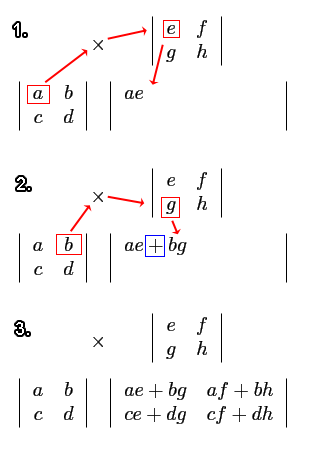
\includegraphics[scale=0.5]{multi_mat.png}\newline
On admet aussi que 
$$\begin{bmatrix} a & b \\ c & d \end{bmatrix} = \begin{bmatrix}e & f \\g & h \end{bmatrix} \Leftrightarrow \left\{\begin{array}{l} a=e\\ b = f \\ c = g \\ d = h \end{array}\right.$$
On note
$$A\times A = A^2$$
pour $A \in \mathscr{M}_2(\R)$
\section{Préliminaires}
\begin{enumerate}
\item 
On note 
$$A = \begin{bmatrix} 2 & -1 \\ 0 & 3 \end{bmatrix}$$
$$B = \begin{bmatrix} 0 & 2  \\ 4 & 1 \end{bmatrix}$$
Calculer $A+B$\newline
Calculer ensuite $A\times B$ et $B\times A$. Que remarquez-vous ?\newline

On dit que le produit matriciel n'est pas commutatif
\item On note 
$$O_2 = \begin{bmatrix} 0 & 0 \\ 0 & 0 \end{bmatrix}$$
Soit $M = \begin{bmatrix} a & b \\ c& d \end{bmatrix}$. Montrer que 
$$M + O_2 = M$$
\item Soit $\lambda \in \R$. Montrer que 
$$\lambda O_2 = O_2$$
\item Soit $M = \begin{bmatrix} a & b \\ c & d\end{bmatrix}$. Montrer que 
$$M\times O_2 = O_2$$
$$O_2 \times M = O_2$$
$O_2$ est l'élément neutre pour l'addition matricielle
\item On note 
$$A = \begin{bmatrix} 1 & -2\\ -2 & 4\end{bmatrix}$$
$$B = \begin{bmatrix} 2 & 4\\ 1 & 2\end{bmatrix}$$
Calculer $A \times B$\newline

On notera que l'on peut avoir $M\times M' = O_2$ avec $M \neq O_2$ et $M' \neq O_2$
\item On note 
$$I_2 = \begin{bmatrix} 1 & 0 \\ 0 & 1 \end{bmatrix}$$
Soit $M = \begin{bmatrix} a & b \\ c & d \end{bmatrix}$. Montrer que 
$$M\times I_2 = M$$
et 
$$I_2 \times M = M$$
$I_2$ est l'élément neutre pour la multiplication matricielle
\end{enumerate}
On admettra les résultats suivants : pour tout $A,B,C \in \mathscr{M}_2(\R)$ et $\lambda \in \R$
$$\boxed{A\times(B+C) = A \times B + A \times C}$$
$$\boxed{(A\times B)\times C = A\times(B\times C)}$$
$$\boxed{A \times (\lambda B) = \lambda(A\times B)}$$
\section{Inverse d'une matrice carrée d'ordre 2}
On dit que $A \in \mathscr{M}_2(\R)$ est inversible s'il existe $B \in \mathscr{M}_2(\R)$ telle que $$A\times B = B \times A = I_2$$
B est alors appelée inverse de $A$
\begin{enumerate}
\item Montrer que $O_2$ n'est pas inversible. \emph{(Indication : on pourra utiliser le résultat de la question 1.4)}
\item Montrer que si 
$$A \times B = B \times A = I_2$$
$$A \times C = C \times A = I_2$$
alors 
$$B = C$$
(on parle d'unicité de l'inverse). Ainsi si $A$ est inversible, on note $A^{-1}$ l'unique matrice telle que $$A\times A^{-1} = A^{-1} \times A = I_2$$
\item Soient 
$$A = \begin{bmatrix} a & b \\ c & d\end{bmatrix}$$
$$X = \begin{bmatrix} x & y \\ z & t\end{bmatrix}$$
($a,b,c,d$ sont connues et $x,y,z,t$ sont les inconnues)\newline

Calculer $$A\times X$$
\item On veut résoudre $A\times X = I_2$. Montrer que cette équation est équivalente au système 
\begin{empheq}[left=(S_1) : \empheqlbrace]{gather}
ax + zb = 1\\
ay + bt = 0\\
cx + dz = 0\\
cy + dt = 1
\end{empheq}
Montrer alors que $a \times (4) - c\times (2)$ permet d'obtenir l'équation 
$$(ad-bc)t=a$$
Montrer alors qu'en faisant $b\times (4) - d\times (2)$ puis $c\times (1) - a \times (3)$ et $d\times (1) - b \times (3)$, on obtient le système 
 \begin{empheq}[left=(S_2) : \empheqlbrace]{gather}
(ad - bc)t = a\\
(bc - ad)y = b\\
(bc - ad)z = c\\
(ad - bc)x = d
\end{empheq}
On suppose, pour l'instant, que $ad - bc \neq 0$. Montrer alors que $A$ est inversible et exprimer $A^{-1}$\newline

On suppose maintenant que $ad - bc = 0$. Déduire du système $(S_2)$ que $AX = I_2$ implique $A = O_2$. En déduire que $A$ n'est alors pas inversible.\newline

Ainsi 
$$\boxed{\begin{bmatrix} a & b \\ c & d\end{bmatrix} \text{ inversible} \Leftrightarrow ad-bc \neq 0}$$
Pour $M = \begin{bmatrix} a & b \\ c & d\end{bmatrix}$, on appelle déterminant de $A$ et on note $\det(M)$ le nombre 
$$\det(M) = ad - bc$$
$$\boxed{M \text{ inversible} \Leftrightarrow \det(M) \neq 0}$$
\item A l'aide de la question précédente, exprimer $A^{-1}$ sous la forme 
$$A^{-1} = \frac{1}{\det(A)} B$$
où $B \in \mathscr{M}_2(\R)$ (on exprimera $B$)
\item On note 
$$A = \begin{bmatrix} 3 & 4\\ 1 & 2\end{bmatrix}$$
Montrer que $A$ est inversible et exprimer $A^{-1}$
\end{enumerate}
\section{Quelques propriétés du déterminant}
\begin{enumerate}
\item Soit 
$$A = \begin{bmatrix} a & b \\ c & d\end{bmatrix}$$
$$B = \begin{bmatrix} e & f \\ g & h\end{bmatrix}$$
Après avoir calculé $A\times B$ et $B\times A$ montrer que $$\det(A\times B) = \det(B \times A) = \det(A)\times\det(B)$$
\item En déduire que si $A\in\mathscr{M}_2(\R)$ est inversible alors 
$$\det(A^{-1}) = \frac{1}{\det(A)}$$
\emph{(Indication : on pourra commencer par montrer que $\det(I_2) = 1$)}
\item Soit $A\in\mathscr{M}_2(\R)$ et $\lambda \in \R$. Montrer que 
$$\det(\lambda A) = \lambda^2 \det(A)$$
\item Soient $A,B \in \mathscr{M}_2(\R)$ et $P\in\mathscr{M}_2(\R)$ inversible. On suppose 
$$A = PBP^{-1}$$
Montrer alors que $\det(A) = \det(B)$
\end{enumerate}
\section{Trace d'une matrice}
Soit $A = \begin{bmatrix}a & b \\ c & d\end{bmatrix}$, on appelle trace de $A$ et on note $Tr(A)$ le nombre $$Tr(A) = a + d$$
\begin{enumerate}
\item Soit $A$ et $B$ dans $\mathscr{M}_2(\R)$, ainsi que $\lambda \in \R$. Montrer que $$Tr(A+B) = Tr(A) + Tr(B)$$ et $$Tr(\lambda A) = \lambda Tr(A)$$
\item Soit $A$ et $B$ dans $\mathscr{M}_2(\R)$, montrer que $$Tr(AB) = Tr(BA)$$ \emph{(Indication : on pourra écrire les matrices avec les coefficients et développer comme des bourrins)}
\item Soient $A,B \in \mathscr{M}_2(\R)$ et $P\in\mathscr{M}_2(\R)$ inversible. On suppose 
$$A = PBP^{-1}$$
Montrer alors que $Tr(A) = Tr(B)$
\end{enumerate}
\section{Transposée d'une matrice}
Soit $A = \begin{bmatrix} a & b \\ c & d \end{bmatrix}$. On appelle transposée de $A$ et on note $^tA$ la matrice 
$$^tA = \begin{bmatrix} a & c \\ b & d \end{bmatrix}$$
\begin{enumerate}
\item Soit $A\in \mathscr{M}_2(\R)$. Montrer que $$Tr(^tA)=Tr(A)$$
\item Montrer que $$\det(^tA) = \det(A)$$
\item Soit $A,B\in \mathscr{M}_2(\R)$. Montrer que $$^t(A\times B) = ^tB\times ^tA$$
\item On suppose $A$ inversible. Montrer alors que $$(^tA)^{-1} = ^t(A^{-1})$$ (il faut montrer que la transposée de l'inverse, bah c'est l'inverse de la transposée)
\item Calculer $^tA\times A$ (en fonction des coefficients de $A$)
\end{enumerate}
\section{Représentation de vecteurs}
Soit $\vv{u}$ et $\vv{v}$ deux vecteurs. $$\vv{u} \covec{a}{c}$$$$\vv{v} \covec{b}{d}$$On note alors $$\text{Mat}(\vv{u},\vv{v}) = \begin{bmatrix} a & b \\ c & d\end{bmatrix}$$
\begin{enumerate}
\item Exprimer $^t\text{Mat}(\vv{u},\vv{v})\times \text{Mat}(\vv{u},\vv{v})$ en fonction de $||\vv{u}||$, $||\vv{v}||$ et $\vv{u} \cdot \vv{v}$
\item R.O.C. Après avoir rappeler la définition de colinéarité entre deux vecteurs, démontrer la condition de colinéarité en fonction des coefficients
\item Que dire de $\vv{u}$ et $\vv{v}$ si $\text{Mat}(\vv{u},\vv{v})$ n'est pas inversible
\end{enumerate}
\center{FIN DU SUJET}
\flushleft
\emph{Les matrices se généralisent à des tailles $n$, voire même à des matrices à $n$ lignes et $p$ colonnes. De plus, la plupart des résultats prouvés ici se généralisent.}
\end{document}